\chapter{曲面坐标系的方程}

\begin{flushright}
\textit{“不以规矩，不能成方圆。”——《孟子·离娄上》}
\footnote{圆和球的边界要靠贴住边界的坐标.柱坐标和球坐标就是这里的规和矩.}
\end{flushright}

正交曲线坐标里的尺度因子、梯度、散度和拉普拉斯算子已经在第~\ref{ch:prelim}~章推导过.这一章用那些公式,在圆柱、圆盘和球面边界上做分离变量.球函数和典型边值问题见~\cite{jackson,morse,wangzhuxi,ivrii}.

\section{柱坐标系下的分离变量法}
\idx{柱坐标}{zhuzuobiao}
\label{sec:cylindrical}

圆形边界在直角坐标里是 $x^2+y^2=a^2$.若试 $V=X(x)Y(y)$,边界上 $X(x)Y(\sqrt{a^2-x^2})=0$ 拆不成只约束 $X$ 的条件和只约束 $Y$ 的条件.改用极坐标以后,同一条边界就是 $\rho=a$,乘积解的两个因子可以各自去满足边界.

与 $z$ 无关时,\eqref{eq:laplace-cyl}退化为
\begin{equation}
  \frac{\partial^2 V}{\partial\rho^2}
  +\frac{1}{\rho}\frac{\partial V}{\partial\rho}
  +\frac{1}{\rho^2}\frac{\partial^2 V}{\partial\phi^2}
  =0.
  \label{eq:polar-laplace}
\end{equation}
设 $V=R(\rho)\Phi(\phi)$,除以 $R\Phi$ 再乘 $\rho^2$,
\begin{equation}
  \frac{\rho}{R}\frac{\mathrm{d}}{\mathrm{d}\rho}
    \Bigl(\rho\frac{\mathrm{d}R}{\mathrm{d}\rho}\Bigr)
  =-\frac{1}{\Phi}\frac{\mathrm{d}^2\Phi}{\mathrm{d}\phi^2}
  =m^2.
\end{equation}
左右只依赖各自的自变量,所以等于同一个常数.这里写成 $m^2$,是为了让角向方程的周期解取正频率.

$\phi$ 增加 $2\pi$ 回到同一点,$\Phi(\phi+2\pi)=\Phi(\phi)$.于是
\begin{equation}
  \Phi''+m^2\Phi=0,
\end{equation}
$m=0,1,2,\ldots$,本征函数是 $1$,以及 $\cos(m\phi)$ 和 $\sin(m\phi)$.$m$ 不是任意实数,单值性把它离散化,作用和固定端把弦的波数离散化相同.

径向方程是欧拉方程
\begin{equation}
  \rho^2 R''+\rho R'-m^2 R=0.
\end{equation}
令 $\rho=e^{s}$,则 $\rho R_{\rho}=R_s$, $\rho^2 R_{\rho\rho}=R_{ss}-R_s$,代入得 $R_{ss}-m^2 R=0$.
$m\geq 1$ 时
\begin{equation}
  R=A\rho^{m}+C\rho^{-m}.
\end{equation}
$m=0$ 时 $R_{ss}=0$,
\begin{equation}
  R=C_0+D_0\ln\rho.
\end{equation}
$\rho^{m}$ 在无穷远处增长,$\rho^{-m}$ 和 $\ln\rho$ 在原点发散.区域包不包原点、包不包无穷远,决定哪一组系数必须为零.

外部区域 $\rho>a$ 的一般解是
\begin{equation}
\begin{aligned}
  V={}&C_0+D_0\ln\rho \\
  &+\sum_{m=1}^{\infty}\Bigl[
      (A_m\rho^{m}+C_m\rho^{-m})\cos(m\phi)
      +(B_m\rho^{m}+D_m\rho^{-m})\sin(m\phi)
    \Bigr].
\end{aligned}
\label{eq:polar-general}
\end{equation}
内部区域 $\rho<a$ 则丢掉 $\ln\rho$ 和 $\rho^{-m}$.

\subsection{均匀电场中的导体圆柱}

\begin{figure}[htb]
  \centering
  \begin{tikzpicture}[font=\small, >=Stealth,
    vec/.style={-{Stealth[length=2mm]}, line width=0.7pt}]
  \draw[gray!35, thin] (-2.6,0) -- (2.6,0) node[right] {$x$};
  \draw[gray!35, thin] (0,-1.9) -- (0,1.9) node[above] {$y$};
  \fill[blue!8] (0,0) circle (0.85);
  \draw[blue!70!black, thick] (0,0) circle (0.85);
  \node at (0,0) {导体};
  \foreach \y in {-1.35,-0.45,0.45,1.35} {
    \draw[vec, gray!80] (-2.45,\y) -- (-1.15,\y);
    \draw[vec, gray!80] (1.15,\y) -- (2.45,\y);
  }
  \draw[vec, red!70!black] (0.85,0) -- (1.55,0) node[midway, above] {$2E_0$};
  \draw[vec, red!70!black] (-1.55,0) -- (-0.85,0);
  \node[font=\scriptsize, gray] at (2.05,1.55) {$\mathbf{E}_0$};
  \node[font=\scriptsize] at (0,-1.55) {$r=a$};
\end{tikzpicture}

  \caption{均匀电场中的中性导体圆柱.远处场恢复为 $\mathbf{E}_0$,表面与外场对齐的两点法向场增强到 $2E_0$.}
  \label{fig:cylinder-field}
\end{figure}

半径为 $a$ 的无限长导体圆柱放在垂直于轴的均匀电场 $\mathbf{E}_0$ 里.取轴为 $z$,$x$ 轴平行于 $\mathbf{E}_0$.导体以外没有电荷,势满足\eqref{eq:polar-laplace}.导体是等势体,把这个常数选成零,
\begin{equation}
  V(a,\phi)=0.
\end{equation}
远处 $E_x\to E_0$, $E_y\to 0$,均匀场的势是 $-E_0 x=-E_0\rho\cos\phi$.若圆柱单位长度还带电 $q_0$,远场再加一项对数,
\begin{equation}
  V(\rho,\phi)\sim
  -\frac{q_0}{2\pi\varepsilon_0}\ln\rho
  -E_0\rho\cos\phi
  \qquad(\rho\to\infty).
\end{equation}
可加常数已经由导体零势定掉.

把\eqref{eq:polar-general}放上 $V(a,\phi)=0$.傅里叶系数各自为零,
\begin{equation}
  C_0+D_0\ln a=0,
  \qquad
  C_m=-a^{2m}A_m,
  \qquad
  D_m=-a^{2m}B_m.
\end{equation}
每一个增长的径向幂都配上一个衰减项,使它们在 $\rho=a$ 上抵消.

远场最高只到 $\rho^1$,所以 $m\geq 2$ 的 $A_m,B_m$ 必须是零,连带的 $C_m,D_m$ 也是零.远场没有 $\sin\phi$,故 $B_1=D_1=0$.余弦的一次项要再现 $-E_0\rho\cos\phi$,故 $A_1=-E_0$, $C_1=E_0 a^2$.对数项的系数是 $D_0=-q_0/(2\pi\varepsilon_0)$,于是 $C_0+D_0\ln\rho=D_0\ln(\rho/a)$.合起来
\begin{equation}
  V(\rho,\phi)
  =\frac{q_0}{2\pi\varepsilon_0}\ln\frac{a}{\rho}
  -E_0\Bigl(\rho-\frac{a^2}{\rho}\Bigr)\cos\phi,
  \qquad\rho\geq a.
  \label{eq:cylinder-potential}
\end{equation}

\begin{example}
中性圆柱的表面电场.
\end{example}
\begin{solution}
$q_0=0$ 时
\begin{equation}
  V=-E_0\Bigl(\rho-\frac{a^2}{\rho}\Bigr)\cos\phi.
\end{equation}
在 $\rho=a$ 上,$\rho-a^2/\rho=0$,导体保持零势.$\rho\to\infty$ 时修正项消失,$V\sim -E_0\rho\cos\phi$.径向电场
\begin{equation}
  E_{\rho}=-\frac{\partial V}{\partial\rho}
  =E_0\Bigl(1+\frac{a^2}{\rho^2}\Bigr)\cos\phi.
\end{equation}
表面上 $E_{\rho}=2E_0\cos\phi$.$\phi=0$ 和 $\phi=\pi$ 两点,法向场的大小都是背景场的两倍,电击穿首先从这里开始.$\phi=\pm\pi/2$ 时 $\cos\phi=0$,中性圆柱的势在这两条射线上处处等于导体的势.
\end{solution}

\subsection{圆内的边值}

\begin{example}
圆盘 $\rho<a$ 的边界上 $V(a,\phi)=V_0\cos\phi$,盘内无电荷,势在圆心有限.
\end{example}
\begin{solution}
内部解丢掉负幂和对数,
\begin{equation}
  V=A_0+\sum_{m=1}^{\infty}\rho^{m}(A_m\cos(m\phi)+B_m\sin(m\phi)).
\end{equation}
边界只有 $\cos\phi$,所以只留下 $m=1$ 的余弦项,$A_1 a=V_0$,
\begin{equation}
  V(\rho,\phi)=V_0\frac{\rho}{a}\cos\phi=V_0\frac{x}{a}.
\end{equation}
它是直角坐标里的线性函数,拉普拉斯算子当然是零.圆形边界把这个简单解从傅里叶级数里挑了出来.
\end{solution}

\subsection{有限圆柱}
$\rho$ 和 $z$ 都有边界时,分离常数落到贝塞尔方程上.考虑稳态温度:圆柱 $0\leq\rho<a$, $0\leq z\leq L$,侧面和底面保持零度,顶面给定轴对称分布 $f(\rho)$,
\begin{equation}
  \nabla^2 T=0,
  \qquad
  T(a,z)=0,
  \qquad
  T(\rho,0)=0,
  \qquad
  T(\rho,L)=f(\rho).
\end{equation}
$f$ 与 $\phi$ 无关,解也与 $\phi$ 无关.\eqref{eq:laplace-cyl}变成
\begin{equation}
  \frac{1}{\rho}\frac{\partial}{\partial\rho}
    \Bigl(\rho\frac{\partial T}{\partial\rho}\Bigr)
  +\frac{\partial^2 T}{\partial z^2}=0.
\end{equation}
设 $T=R(\rho)Z(z)$.为了让 $R(a)=0$ 而且 $R$ 在轴上有限,分离常数取正,
\begin{equation}
  \frac{1}{\rho R}\frac{\mathrm{d}}{\mathrm{d}\rho}
    \Bigl(\rho\frac{\mathrm{d}R}{\mathrm{d}\rho}\Bigr)
  =-k^2
  =\frac{1}{Z}\frac{\mathrm{d}^2 Z}{\mathrm{d}z^2}.
\end{equation}
径向方程是 $0$ 阶贝塞尔方程.令 $\xi=k\rho$,则
\begin{equation}
  \xi^2\frac{\mathrm{d}^2 R}{\mathrm{d}\xi^2}
  +\xi\frac{\mathrm{d}R}{\mathrm{d}\xi}
  +\xi^2 R=0,
\end{equation}
在 $\xi=0$ 有限的解是 $J_0(k\rho)$.侧面 $J_0(ka)=0$,所以
\begin{equation}
  k_m=\frac{j_{0,m}}{a},
  \qquad m=1,2,\ldots,
\end{equation}
$j_{0,m}$ 是 $J_0$ 的第 $m$ 个正零点.轴向方程 $Z''-k_m^2 Z=0$,底面 $Z(0)=0$ 选出
\begin{equation}
  Z=\sinh(k_m z).
\end{equation}
叠加
\begin{equation}
  T(\rho,z)
  =\sum_{m=1}^{\infty} A_m J_0(k_m\rho)\sinh(k_m z).
\end{equation}
顶面 $z=L$ 用贝塞尔族的正交性定系数.权重为 $\rho$ 的模是
\begin{equation}
  \int_0^{a}\rho\, J_0(k_m\rho)^2\,\mathrm{d}\rho
  =\frac{a^2}{2}J_1(k_m a)^2,
\end{equation}
因此
\begin{equation}
  A_m\sinh(k_m L)
  =\frac{2}{a^2 J_1(k_m a)^2}
    \int_0^{a} f(\rho)\, J_0(k_m\rho)\,\rho\,\mathrm{d}\rho.
  \label{eq:cylinder-coeff}
\end{equation}

\begin{example}
顶面温度是常数 $T_0$.
\end{example}
\begin{solution}
用 $\mathrm{d}[u J_1(u)]/\mathrm{d}u=u J_0(u)$,
\begin{equation}
  \int_0^{a}\rho\, J_0(k_m\rho)\,\mathrm{d}\rho
  =\frac{a}{k_m}J_1(k_m a).
\end{equation}
代入\eqref{eq:cylinder-coeff},
\begin{equation}
  A_m
  =\frac{2T_0}{k_m a\, J_1(k_m a)\,\sinh(k_m L)}.
\end{equation}
于是
\begin{equation}
  T(\rho,z)
  =\sum_{m=1}^{\infty}
    \frac{2T_0}{j_{0,m} J_1(j_{0,m})\, \sinh(k_m L)}
    \, J_0(k_m\rho)\sinh(k_m z),
\end{equation}
其中用了 $k_m a=j_{0,m}$.$z=0$ 时每一项都是零;$z=L$ 时双曲正弦之比变成 $1$,剩下的级数就是常数 $T_0$ 的贝塞尔展开.侧面 $\rho=a$ 上 $J_0(k_m a)=0$.
\end{solution}

\section{球坐标系下的分离变量法}
\idx{球坐标}{qiuzuobiao}
\idx{勒让德多项式}{lerangde}
\idx{球谐函数}{qiuxie}
\label{sec:spherical}

球坐标里的拉普拉斯算子是\eqref{eq:laplace-sph}.静电、稳态温度和引力势在无源区域都满足 $\nabla^2 u=0$.设
\begin{equation}
  u(r,\theta,\phi)=R(r)\,\Theta(\theta)\,\Phi(\phi),
\end{equation}
代入后乘 $r^2/(R\Theta\Phi)$,
\begin{equation}
  \frac{1}{R}\frac{\mathrm{d}}{\mathrm{d}r}
    \Bigl(r^2\frac{\mathrm{d}R}{\mathrm{d}r}\Bigr)
  =-\frac{1}{\Theta\sin\theta}\frac{\mathrm{d}}{\mathrm{d}\theta}
      \Bigl(\sin\theta\frac{\mathrm{d}\Theta}{\mathrm{d}\theta}\Bigr)
   -\frac{1}{\Phi\sin^2\theta}\frac{\mathrm{d}^2\Phi}{\mathrm{d}\phi^2}.
  \label{eq:sph-separated}
\end{equation}
左边只依赖 $r$.右边再乘 $\sin^2\theta$ 之后,$\phi$ 的部分可以单独分离出来.

\subsection{方位角}
$\Phi(\phi+2\pi)=\Phi(\phi)$,所以
\begin{equation}
  \frac{1}{\Phi}\frac{\mathrm{d}^2\Phi}{\mathrm{d}\phi^2}=-m^2,
  \qquad
  \Phi=e^{\imath m\phi},
  \qquad m\in\mathbb{Z}.
\end{equation}
$m=0$ 是轴对称情形.把 $-m^2$ 代回\eqref{eq:sph-separated},右边变成只含 $\theta$ 的式子,它必须等于常数.为了让极角方程在 $\theta=0,\pi$ 有有限解,这个常数写成 $\ell(\ell+1)$, $\ell=0,1,2,\ldots$,并且 $|m|\leq\ell$.径向方程于是是
\begin{equation}
  \frac{\mathrm{d}}{\mathrm{d}r}
    \Bigl(r^2\frac{\mathrm{d}R}{\mathrm{d}r}\Bigr)
  -\ell(\ell+1)R=0.
  \label{eq:radial-euler}
\end{equation}
试 $R=r^{\alpha}$,得到 $\alpha(\alpha+1)=\ell(\ell+1)$,两个根是 $\alpha=\ell$ 和 $\alpha=-(\ell+1)$.因此
\begin{equation}
  R(r)=A\, r^{\ell}+B\, r^{-(\ell+1)}.
  \label{eq:radial-power}
\end{equation}
含原点的区域丢掉负幂,外部问题在无穷远处丢掉正幂.

若方程是亥姆霍兹方程 $\nabla^2 u+k^2 u=0$,径向因子改成球贝塞尔函数 $j_{\ell}(kr)$,见特殊函数一章.$k=0$ 时幂次解\eqref{eq:radial-power}就是它的极限.

\subsection{勒让德方程}
极角方程是
\begin{equation}
  \frac{1}{\sin\theta}\frac{\mathrm{d}}{\mathrm{d}\theta}
    \Bigl(\sin\theta\frac{\mathrm{d}\Theta}{\mathrm{d}\theta}\Bigr)
  +\Biggl[\ell(\ell+1)-\frac{m^2}{\sin^2\theta}\Biggr]\Theta=0.
  \label{eq:theta-eq}
\end{equation}
令 $x=\cos\theta$,则 $\mathrm{d}/\mathrm{d}\theta=-\sin\theta\,\mathrm{d}/\mathrm{d}x$,并且
\begin{equation}
  \frac{1}{\sin\theta}\frac{\mathrm{d}}{\mathrm{d}\theta}
    \Bigl(\sin\theta\frac{\mathrm{d}\Theta}{\mathrm{d}\theta}\Bigr)
  =\frac{\mathrm{d}}{\mathrm{d}x}
    \Biggl((1-x^2)\frac{\mathrm{d}\Theta}{\mathrm{d}x}\Biggr).
\end{equation}
\eqref{eq:theta-eq}变成连带勒让德方程
\begin{equation}
  (1-x^2)\frac{\mathrm{d}^2 P}{\mathrm{d}x^2}
  -2x\frac{\mathrm{d}P}{\mathrm{d}x}
  +\Biggl[\ell(\ell+1)-\frac{m^2}{1-x^2}\Biggr]P=0,
  \label{eq:associated-legendre}
\end{equation}
其中 $P(x)=\Theta(\arccos x)$,$x\in[-1,1]$.

$m=0$ 时它退化为勒让德方程
\begin{equation}
  (1-x^2)P_{\ell}''-2x P_{\ell}'+\ell(\ell+1)P_{\ell}=0.
  \label{eq:legendre-ode}
\end{equation}
在 $x=\pm 1$ 有限的解是 $\ell$ 次多项式 $P_{\ell}(x)$.级数解在端点一般有对数奇性,只有 $\ell$ 是非负整数时级数截成多项式.

\subsection{罗德里格斯公式}
\begin{equation}
  P_{\ell}(x)
  =\frac{1}{2^{\ell}\ell!}
    \frac{\mathrm{d}^{\ell}}{\mathrm{d}x^{\ell}}(x^2-1)^{\ell}.
  \label{eq:rodrigues}
\end{equation}
$(x^2-1)^{\ell}$ 是 $2\ell$ 次多项式,求导 $\ell$ 次后是 $\ell$ 次多项式,并且 $P_{\ell}(1)=1$.

\begin{figure}[htb]
  \centering
  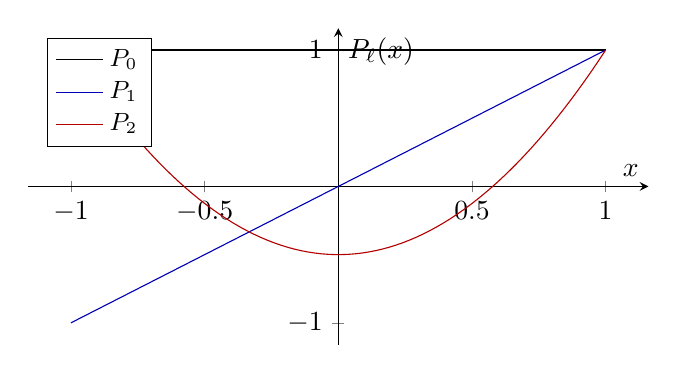
\begin{tikzpicture}
\begin{axis}[
    width=0.78\textwidth,
    height=5.6cm,
    xlabel={$x$},
    ylabel={$P_{\ell}(x)$},
    domain=-1:1,
    samples=80,
    legend pos=north west,
    legend style={font=\small},
    axis lines=middle,
    enlargelimits=0.08,
  ]
  \addplot[black] {1};
  \addplot[blue!70!black] {x};
  \addplot[red!70!black] {0.5*(3*x^2-1)};
  \legend{$P_0$,$P_1$,$P_2$}
\end{axis}
\end{tikzpicture}

  \caption{$P_0$, $P_1$, $P_2$.$P_{\ell}$ 在 $(-1,1)$ 里有 $\ell$ 个零点,并且 $P_{\ell}(1)=1$.}
  \label{fig:legendre}
\end{figure}

\begin{example}
用罗德里格斯公式算 $P_0,P_1,P_2$.
\end{example}
\begin{solution}
$\ell=0$ 时没有求导,$P_0=1$.$\ell=1$,
\begin{equation}
  P_1=\frac{1}{2}\frac{\mathrm{d}}{\mathrm{d}x}(x^2-1)=x.
\end{equation}
$\ell=2$, $(x^2-1)^2=x^4-2x^2+1$,二阶导数是 $12x^2-4$,
\begin{equation}
  P_2=\frac{1}{8}(12x^2-4)=\frac{1}{2}(3x^2-1).
\end{equation}
三者都满足 $P_{\ell}(1)=1$.把 $P_2$ 代入\eqref{eq:legendre-ode}: $P_2'=3x$, $P_2''=3$,
\begin{equation}
  (1-x^2)\cdot 3-2x\cdot 3x+6\cdot\frac{1}{2}(3x^2-1)
  =3-3x^2-6x^2+9x^2-3=0.
\end{equation}
\end{solution}

\subsection{正交性与生成函数}
\eqref{eq:legendre-ode}写成自伴形式
\begin{equation}
  \frac{\mathrm{d}}{\mathrm{d}x}\bigl[(1-x^2)P_{\ell}'\bigr]+\ell(\ell+1)P_{\ell}=0.
\end{equation}
$\ell\neq\ell'$ 时,用 $P_{\ell'}$ 和 $P_{\ell}$ 分别乘对方的方程再相减,从 $-1$ 积到 $1$.左边是
\begin{equation}
  \Bigl[(1-x^2)\bigl(P_{\ell'}P_{\ell}'-P_{\ell}P_{\ell'}'\bigr)\Bigr]_{-1}^{1}=0,
\end{equation}
因为 $1-x^2$ 在端点为零,而勒让德多项式的导数在端点有限.因此
\begin{equation}
  \int_{-1}^{1} P_{\ell}(x)P_{\ell'}(x)\,\mathrm{d}x=0,
  \qquad\ell\neq\ell'.
\end{equation}

生成函数
\begin{equation}
  \frac{1}{\sqrt{1-2xt+t^2}}
  =\sum_{\ell=0}^{\infty} P_{\ell}(x)\, t^{\ell},
  \qquad |t|<1.
  \label{eq:legendre-generating}
\end{equation}
$t=0$ 时左边是 $1$,所以 $P_0=1$.对 $t$ 求导再令 $t=0$,得到 $P_1=x$.把 $x=1$ 代入,左边是 $1/(1-t)=\sum t^{\ell}$,因此每个 $P_{\ell}(1)=1$.

模由生成函数的平方积分定出.令
\begin{equation}
  G(x,t)=\frac{1}{\sqrt{1-2xt+t^2}}.
\end{equation}
正交性使交叉项消失,
\begin{equation}
  \int_{-1}^{1} G(x,t)^2\,\mathrm{d}x
  =\sum_{\ell=0}^{\infty} t^{2\ell}\int_{-1}^{1} P_{\ell}(x)^2\,\mathrm{d}x.
\end{equation}
左边直接积,
\begin{equation}
  \int_{-1}^{1}\frac{\mathrm{d}x}{1-2xt+t^2}
  =\frac{1}{t}\ln\frac{1+t}{1-t}
  =2\sum_{\ell=0}^{\infty}\frac{t^{2\ell}}{2\ell+1}.
\end{equation}
比较 $t^{2\ell}$ 的系数,
\begin{equation}
  \int_{-1}^{1} P_{\ell}(x)^2\,\mathrm{d}x=\frac{2}{2\ell+1}.
  \label{eq:legendre-norm}
\end{equation}
于是 $[-1,1]$ 上的勒让德级数是
\begin{equation}
  f(x)=\sum_{\ell=0}^{\infty} a_{\ell} P_{\ell}(x),
  \qquad
  a_{\ell}=\frac{2\ell+1}{2}\int_{-1}^{1} f(x)P_{\ell}(x)\,\mathrm{d}x.
  \label{eq:legendre-series}
\end{equation}

对\eqref{eq:legendre-generating}作 $\partial/\partial t$,用 $(1-2xt+t^2)\partial G/\partial t=(x-t)G$,比较 $t^{\ell}$ 的系数,得到递推
\begin{equation}
  (\ell+1)P_{\ell+1}(x)=(2\ell+1)x P_{\ell}(x)-\ell P_{\ell-1}(x).
  \label{eq:legendre-recurrence}
\end{equation}
由 $P_0$ 和 $P_1$ 可以逐个写出后面的多项式,不必每次都求导.

\begin{example}
把 $f(x)=x^2$ 展开成勒让德级数.
\end{example}
\begin{solution}
$P_2=\half(3x^2-1)$,所以 $x^2=\tfrac{2}{3}P_2+\tfrac{1}{3}P_0$.用系数公式核对.$a_0=\half\int_{-1}^{1}x^2\,\mathrm{d}x=\tfrac{1}{3}$.
\begin{equation}
  a_2=\frac{5}{2}\int_{-1}^{1} x^2\cdot\frac{3x^2-1}{2}\,\mathrm{d}x
  =\frac{5}{2}\cdot\frac{4}{15}
  =\frac{2}{3}.
\end{equation}
更高阶与 $x^2$ 正交,系数是零.这个展开在球面上就是轴对称势的 $\ell=0$ 和 $\ell=2$ 两项.
\end{solution}

\subsection{连带勒让德函数}
$m\geq 0$ 时,连带勒让德函数由 $P_{\ell}$ 定义,
\begin{equation}
  P_{\ell}^{m}(x)
  =(-1)^{m}(1-x^2)^{m/2}\frac{\mathrm{d}^{m}}{\mathrm{d}x^{m}}P_{\ell}(x).
  \label{eq:assoc-def}
\end{equation}
前面的 $(-1)^{m}$ 是 Condon--Shortley 相位.负阶由
\begin{equation}
  P_{\ell}^{-m}(x)
  =(-1)^{m}\frac{(\ell-m)!}{(\ell+m)!}P_{\ell}^{m}(x)
\end{equation}
定出,这样 $|m|\leq\ell$ 的全部函数都归到 $m\geq 0$ 的导数上.$m>\ell$ 时 $\ell$ 次多项式的 $m$ 阶导数是零.

\begin{example}
$P_2^{1}$ 与 $P_1^{1}$.
\end{example}
\begin{solution}
$P_1=x$,所以 $P_1^{1}=-(1-x^2)^{1/2}=-\sin\theta$.$P_2' =3x$,
\begin{equation}
  P_2^{1}(x)=-3x\sqrt{1-x^2}=-3\cos\theta\sin\theta.
\end{equation}
$x=\pm 1$ 时因子 $\sqrt{1-x^2}$ 是零,极点上 $m\neq 0$ 的连带函数消失,方位角才可以不确定.
\end{solution}

固定 $m$ 时,它们在 $[-1,1]$ 上正交,
\begin{equation}
  \int_{-1}^{1} P_{\ell}^{m}(x)P_{\ell'}^{m}(x)\,\mathrm{d}x
  =\frac{2}{2\ell+1}\frac{(\ell+m)!}{(\ell-m)!}\,\delta_{\ell\ell'}.
  \label{eq:assoc-norm}
\end{equation}
$m=0$ 时回到\eqref{eq:legendre-norm}.同一 $\ell$ 的递推是
\begin{equation}
  (\ell-m+1)P_{\ell+1}^{m}(x)
  =(2\ell+1)x P_{\ell}^{m}(x)
  -(\ell+m)P_{\ell-1}^{m}(x).
\end{equation}

\subsection{球谐函数}
球面上的归一化本征函数是球谐函数
\begin{equation}
  Y_{\ell}^{m}(\theta,\phi)
  =N_{\ell m}\, P_{\ell}^{m}(\cos\theta)\, e^{\imath m\phi},
  \label{eq:spherical-harmonic}
\end{equation}
\begin{equation}
  N_{\ell m}
  =\sqrt{\frac{2\ell+1}{4\pi}\frac{(\ell-m)!}{(\ell+m)!}}.
\end{equation}
相位已经放在\eqref{eq:assoc-def}里,这里不再乘 $(-1)^{m}$.$m<0$ 时把负阶的 $P_{\ell}^{m}$ 代进同一公式.面积元 $\mathrm{d}\Omega=\sin\theta\,\mathrm{d}\theta\,\mathrm{d}\phi$,
\begin{equation}
  \int Y_{\ell}^{m}\,\overline{Y_{\ell'}^{m'}}\,\mathrm{d}\Omega
  =\delta_{\ell\ell'}\delta_{mm'}.
\end{equation}
前几个是
\begin{align}
  Y_0^{0}&=\frac{1}{\sqrt{4\pi}}, \\
  Y_1^{0}&=\sqrt{\frac{3}{4\pi}}\cos\theta, \\
  Y_1^{\pm 1}&=\mp\sqrt{\frac{3}{8\pi}}\sin\theta\, e^{\pm\imath\phi}.
\end{align}
$Y_1^{0}$ 的归一化可以手算:方位角积出 $2\pi$,再令 $u=\cos\theta$,
\begin{equation}
  \int |Y_1^{0}|^2\,\mathrm{d}\Omega
  =\frac{3}{4\pi}\cdot 2\pi\int_{-1}^{1} u^2\,\mathrm{d}u
  =\frac{3}{2}\cdot\frac{2}{3}=1.
\end{equation}

球面上的函数展开成
\begin{equation}
  F(\theta,\phi)
  =\sum_{\ell=0}^{\infty}\sum_{m=-\ell}^{\ell}
    c_{\ell m} Y_{\ell}^{m}(\theta,\phi),
  \qquad
  c_{\ell m}=\int F\,\overline{Y_{\ell}^{m}}\,\mathrm{d}\Omega.
\end{equation}
轴对称时只剩 $m=0$,而 $Y_{\ell}^{0}$ 正比于 $P_{\ell}(\cos\theta)$,展开就是\eqref{eq:legendre-series}.

\subsection{均匀电场中的导体球}

\begin{figure}[htb]
  \centering
  \begin{tikzpicture}[font=\small, >=Stealth,
    vec/.style={-{Stealth[length=2mm]}, line width=0.7pt}]
  \draw[gray!35, thin] (0,-2.15) -- (0,2.35) node[above] {$z$};
  \draw[gray!35, thin] (-2.2,0) -- (2.2,0) node[right] {$x$};
  \fill[blue!8] (0,0) circle (0.9);
  \draw[blue!70!black, thick] (0,0) circle (0.9);
  \foreach \x in {-1.2,-0.4,0.4,1.2} {
    \draw[vec, gray!75] (\x,-2.05) -- (\x,-1.15);
    \draw[vec, gray!75] (\x,1.15) -- (\x,2.05);
  }
  \draw[vec, red!70!black] (0,0.9) -- (0,1.7) node[midway, right] {$3E_0$};
  \draw[vec, red!70!black] (0,-1.7) -- (0,-0.9);
  \node at (0,0) {导体};
  \node[font=\scriptsize, gray] at (1.55,1.85) {$\mathbf{E}_0$};
\end{tikzpicture}

  \caption{均匀电场中的中性导体球.极点上的法向场是 $3E_0$,赤道上法向场为零.}
  \label{fig:sphere-field}
\end{figure}

半径为 $a$ 的导体球放在沿 $z$ 轴的均匀电场 $\mathbf{E}_0$ 里,球面电位取为零.球外 $\nabla^2 V=0$,轴对称,所以
\begin{equation}
  V(r,\theta)
  =\sum_{\ell=0}^{\infty}
    \bigl(A_{\ell} r^{\ell}+B_{\ell} r^{-(\ell+1)}\bigr) P_{\ell}(\cos\theta).
\end{equation}
远处 $V\sim -E_0 z=-E_0 r\cos\theta=-E_0 r P_1(\cos\theta)$,因此 $A_1=-E_0$,其余 $A_{\ell}=0$.负幂在无穷远处自己消失,可以保留.球面 $V(a,\theta)=0$ 要求每一项的两个径向系数抵消,
\begin{equation}
  B_1=-A_1 a^{3}=E_0 a^{3},
\end{equation}
其它 $B_{\ell}=0$.于是
\begin{equation}
  V(r,\theta)
  =-E_0\Bigl(r-\frac{a^3}{r^2}\Bigr)\cos\theta,
  \qquad r\geq a.
  \label{eq:sphere-potential}
\end{equation}

\begin{example}
球面上的电场,以及它和圆柱结果的差别.
\end{example}
\begin{solution}
\begin{equation}
  E_r=-\frac{\partial V}{\partial r}
  =E_0\Bigl(1+\frac{2a^3}{r^3}\Bigr)\cos\theta.
\end{equation}
$r=a$ 时 $E_r=3E_0\cos\theta$.两极是 $3E_0$,不是圆柱表面上的 $2E_0$.赤道 $\theta=\pi/2$ 上 $\cos\theta=0$,法向场为零.$r=a$ 时括号 $r-a^3/r^2$ 是零,球面保持零势.感应面电荷 $\sigma=\varepsilon_0 E_r=3\varepsilon_0 E_0\cos\theta$,北半球与南半球反号,总电荷是零.
\end{solution}

\subsection{球面上给定的电位}

\begin{example}
球内势在原点有限,球面电位是 $V(a,\theta)=V_0\cos\theta$.
\end{example}
\begin{solution}
内部丢掉 $r^{-(\ell+1)}$.边界是 $P_1$,只留下
\begin{equation}
  V(r,\theta)=A_1 r\cos\theta,
  \qquad A_1 a=V_0,
\end{equation}
\begin{equation}
  V(r,\theta)=V_0\frac{r}{a}\cos\theta=V_0\frac{z}{a}.
\end{equation}
球外、无穷远处趋于零的对应问题丢掉 $r^{\ell}$,
\begin{equation}
  V(r,\theta)=V_0\frac{a^2}{r^2}\cos\theta,
  \qquad r\geq a.
\end{equation}
一般的轴对称球面电位 $f(\theta)$ 先按 $x=\cos\theta$ 作勒让德展开,$a_{\ell}$ 用\eqref{eq:legendre-series}.球内是 $\sum a_{\ell}(r/a)^{\ell} P_{\ell}(\cos\theta)$,球外是 $\sum a_{\ell}(a/r)^{\ell+1} P_{\ell}(\cos\theta)$.
\end{solution}

\section{圆盘的泊松公式}
\idx{泊松公式}{bosonggongshi}
圆内拉普拉斯方程的分离已经在柱坐标一节做过:有界解是
\begin{equation}
  u(r,\theta)=\frac{A_0}{2}+\sum_{n=1}^{\infty}r^n\bigl(A_n\cos(n\theta)+C_n\sin(n\theta)\bigr),
  \qquad r<a.
  \label{eq:disk-interior}
\end{equation}
边界 $u(a,\theta)=g(\theta)$ 把系数定成 $g$ 的傅里叶系数再除以 $a^n$.代回去,
\begin{equation}
  u(r,\theta)=\int_0^{2\pi}P(r,\theta-\theta')g(\theta')\,\mathrm{d}\theta',
\end{equation}
核是几何级数
\begin{equation}
  P=\frac{1}{2\pi}\Biggl(1+2\sum_{n=1}^{\infty}\Bigl(\frac{r}{a}\Bigr)^n\cos\bigl(n(\theta-\theta')\bigr)\Biggr).
\end{equation}
公比 $z=(r/a)e^{\imath(\theta-\theta')}$ 的模小于 $1$,求和得到
\begin{equation}
  P(r,\theta-\theta')
  =\frac{1}{2\pi}\frac{a^2-r^2}{a^2-2ar\cos(\theta-\theta')+r^2}.
  \label{eq:poisson-kernel}
\end{equation}
这是圆盘的泊松公式.圆心处 $r=0$,核变成 $1/(2\pi)$,所以
\begin{equation}
  u(0)=\frac{1}{2\pi}\int_0^{2\pi}g(\theta')\,\mathrm{d}\theta',
\end{equation}
圆心的值是边界值的平均.

圆外 $r>a$、无穷远处有界的解丢掉正幂,同一套求和把 $r/a$ 换成 $a/r$,核的分子换成 $r^2-a^2$.$r\to\infty$ 时 $u$ 趋于边界值的同一个平均.

\begin{example}
边界 $g=\cos\theta$,用泊松核核对 $u=(r/a)\cos\theta$.
\end{example}
\begin{solution}
$\cos\theta'$ 对 $\theta'$ 的积分只留下核里 $n=1$ 的余弦.系数是 $(r/a)$,乘上 $\cos\theta$,就是 $u=(r/a)\cos\theta$.它在 $r=a$ 上等于 $\cos\theta$,并且是 $x/a$,调和.
\end{solution}

\section{圆盘的诺伊曼问题}
边界上给定径向导数 $u_r(a,\theta)=h(\theta)$,内部仍然用\eqref{eq:disk-interior}.对 $r$ 求导再令 $r=a$,
\begin{equation}
  h(\theta)=\sum_{n=1}^{\infty}n a^{n-1}\bigl(A_n\cos(n\theta)+C_n\sin(n\theta)\bigr).
\end{equation}
常数项不出现在 $u_r$ 里,所以 $h$ 的平均值必须是零,否则无解.平均值是零时,$n\geq 1$ 的系数除以 $na^{n-1}$,$A_0$ 仍然任意,对应加上常数.解差一个常数,和诺伊曼问题的一般情形一致.

\section{扇形、圆环和带割缝的圆盘}
两条射线 $\theta=0$ 和 $\theta=\alpha$ 上也给定齐次条件时,角向不再以 $2\pi$ 为周期.$\Theta(0)=\Theta(\alpha)=0$ 给出 $\Theta=\sin(n\pi\theta/\alpha)$,径向幂次从整数改成
\begin{equation}
  R=A r^{n\pi/\alpha}+B r^{-n\pi/\alpha}.
\end{equation}
扇形 $r<a$ 丢掉负幂,扇形外部丢掉正幂,环扇形 $a<r<b$ 两项都留.

\begin{example}
半环 $1<r<2$, $0<\theta<\pi$, $\theta=0,\pi$ 和 $r=1$ 上 $u=0$, $u(2,\theta)=\pi-\theta$.
\end{example}
\begin{solution}
$\alpha=\pi$,角向是 $\sin(n\theta)$,径向是 $A_n r^n+B_n r^{-n}$.$r=1$ 上为零要求 $B_n=-A_n$,
\begin{equation}
  u=\sum_{n=1}^{\infty}A_n(r^n-r^{-n})\sin(n\theta).
\end{equation}
$r=2$ 上 $\pi-\theta$ 的正弦系数是
\begin{equation}
  \frac{2}{\pi}\int_0^{\pi}(\pi-\theta)\sin(n\theta)\,\mathrm{d}\theta=\frac{2}{n}.
\end{equation}
因此 $A_n(2^n-2^{-n})=2/n$,
\begin{equation}
  u(r,\theta)=\sum_{n=1}^{\infty}
  \frac{2}{n(2^n-2^{-n})}(r^n-r^{-n})\sin(n\theta).
\end{equation}
\end{solution}

割缝上的边界值如果不是零,先找一个满足方程和割缝条件的特解,差满足齐次割缝条件,再分离变量.割缝 $\theta=\pm\pi$ 上 $x=r\cos\theta=-r$.因此 $1+x$ 在两条缝上都等于 $1-r$,它又是调和函数.若还要求 $r=1$ 上 $u=0$,令 $w=u-(1+x)$,则 $w$ 在缝上为零,在 $r=1$ 上等于 $-1-\cos\theta$.角向区间长度是 $2\pi$,两端为零,本征函数是 $\sin\bigl((n/2)(\theta+\pi)\bigr)$,也就是半整数族.$-1-\cos\theta$ 对 $\theta$ 是偶的,只激发其中的余弦型项.

圆环 $a<r<b$ 上两个圆都给边值时,正幂和负幂都留,$n=0$ 还有 $A+B\ln r$.两个圆上的傅里叶系数各给一个线性方程,解出 $A_n,B_n$.

\section{圆盘和圆柱上的亥姆霍兹方程}
振动膜或定态波满足 $\Delta u+k^2 u=0$.极坐标里分离 $u=R(r)e^{\imath m\phi}$,$m\in\mathbb{Z}$,径向是贝塞尔方程
\begin{equation}
  r^2 R''+r R'+(k^2 r^2-m^2)R=0.
\end{equation}
圆心有界的解是 $J_m(kr)$.圆周 $r=a$ 上 $u=0$ 要求
\begin{equation}
  J_m(ka)=0.
\end{equation}
$J_m$ 的正零点 $j_{m,s}$ 给出 $k_{m,s}=j_{m,s}/a$,每个 $m\geq 1$ 的 $\cos(m\phi)$ 和 $\sin(m\phi)$ 共用这个 $k$.时间因子是 $\cos(ckt)$ 和 $\sin(ckt)$.

有限圆柱上若侧面为零、振动与 $\phi$ 无关,径向仍是 $J_0$,轴向是正弦,分离常数拆成 $k^2=\alpha^2+\beta^2$.侧面条件定 $\alpha$,上下条件定 $\beta$.

\section{调和多项式}
\idx{调和多项式}{tiaoheduoxiangshi}
球内的调和函数若在球心光滑,径向只能是 $r^{\ell}$,$\ell=0,1,2,\ldots$,对应的角向函数是 $\ell$ 次球谐.把它写成 $x,y,z$ 的函数,就是 $\ell$ 次齐次调和多项式.$\ell$ 次齐次多项式的维数是 $\binom{\ell+2}{2}$.任意 $\ell-2$ 次齐次多项式都是某个 $\ell$ 次齐次多项式的拉普拉斯,这个条件用掉 $\binom{\ell}{2}$ 个系数,剩下
\begin{equation}
  \binom{\ell+2}{2}-\binom{\ell}{2}=2\ell+1.
\end{equation}
这和 $m=-\ell,\ldots,\ell$ 的个数一致.前几次的一组基是
\begin{center}
\begin{tabular}{cl}
$\ell$ & 基 \\
$0$ & $1$ \\
$1$ & $x,\; y,\; z$ \\
$2$ & $xy,\; xz,\; yz,\; x^2-y^2,\; x^2-z^2$
\end{tabular}
\end{center}
球外、无穷远处衰减的调和函数把 $r^{\ell}$ 换成 $r^{-(\ell+1)}$.同样这 $2\ell+1$ 个函数除以 $r^{2\ell+1}$ 仍然调和,例如 $\ell=1$ 时是 $x/r^3$, $y/r^3$, $z/r^3$.

\section{球内的波动}
球 $r\leq a$ 内 $u_{tt}=c^2\Delta u$,球面 $u=0$ 或 $u_r=0$.先分离时间,$v_{tt}$ 的角色变成亥姆霍兹方程 $\Delta v+\lambda v=0$,再分离出球谐 $Y_{\ell}^{m}$.径向方程
\begin{equation}
  r^2 R''+2r R'+\bigl(\lambda r^2-\ell(\ell+1)\bigr)R=0
\end{equation}
的有界解是球贝塞尔函数 $j_{\ell}(\sqrt{\lambda}\,r)$.狄利克雷条件是 $j_{\ell}(\sqrt{\lambda}\,a)=0$,诺伊曼条件是它的导数在 $r=a$ 为零.每个零点给一个频率 $\omega=c\sqrt{\lambda}$,时间因子是 $\cos\omega t$ 和 $\sin\omega t$.同一个 $\ell$ 的 $2\ell+1$ 个 $m$ 共用这些频率.

氢原子的库仑问题也是先分离出 $Y_{\ell}^{m}$,径向再要求级数截断.能级 $E_n\propto -1/n^2$ 和简并度 $n^2$ 在特殊函数一章里.

\section{椭圆坐标和抛物坐标}
平面上的共形坐标把拉普拉斯方程变成同一个算子的倍数.椭圆坐标和抛物坐标都来自复解析函数,
\begin{equation}
  x+\imath y=c\cosh(\sigma+\imath\tau),
  \qquad
  x+\imath y=\frac{(\sigma+\imath\tau)^2}{2}.
\end{equation}
尺度因子在两个方向上相等,所以
\begin{equation}
  \Delta u=\frac{1}{h^2}(u_{\sigma\sigma}+u_{\tau\tau}).
\end{equation}
$\Delta u=0$ 就是 $u_{\sigma\sigma}+u_{\tau\tau}=0$,分离变量和直角坐标一样,得到指数或三角函数.亥姆霍兹方程 $\Delta u+k^2 u=0$ 乘上 $h^2$ 之后,分离常数一边是马蒂厄方程,另一边仍是周期的三角方程.把抛物线绕对称轴旋转,或在抛物坐标上再加一个 $z$,就得到三维的抛物坐标和抛物柱坐标,拉普拉斯算子仍然分离.球、圆柱、椭圆、抛物这几族,是三维空间里拉普拉斯算子能够分离的正交坐标.

柱坐标和球坐标的解要先满足拉普拉斯方程,再套边界.勒让德展开的系数要用正交关系算出来.

\begin{problemset}
\renewcommand{\theenumi}{\thechapter.\arabic{enumi}}
\renewcommand{\labelenumi}{\theenumi.}
\item 由位置矢量算出柱坐标和球坐标的尺度因子.说明 $\phi$ 方向的弧长在柱坐标里是 $\rho\,\mathrm{d}\phi$,在球坐标里是 $r\sin\theta\,\mathrm{d}\phi$.

\item 均匀电场 $\mathbf{E}_0$ 垂直于无限长导体圆柱的轴,柱面接地.在柱外求电位,并计算柱面上的电场.说明它为什么是 $2E_0\cos\phi$.

\item 圆盘 $\rho<a$ 的边界电位是 $V_0\cos\phi$.求盘内电位,并在 $\rho=a$ 上核对边界值.

\item 有限圆柱 $0\leq\rho<a$, $0\leq z<b$,侧面和底面电位为零,顶面 $z=b$ 的电位是 $f(\rho)$.写出用 $J_0$ 表示的级数,并把系数写成积分.

\item 用罗德里格斯公式算出 $P_0,P_1,P_2$.验证它们满足勒让德方程,并且 $P_\ell(1)=1$.

\item 均匀电场中的接地导体球,写出球外电位和球面电场.说明表面场是 $3E_0\cos\theta$.

\item 球面 $r=a$ 上的电位是 $V_0\cos^2\theta$.把它展成 $P_0$ 和 $P_2$,分别写出球内和球外的电位.

\item 用泊松核说明圆盘中心的电位是边界值的圆周平均.再对 $g(\theta)=\cos\theta$ 算出盘内电位,与分离变量的结果比较.

\item 圆盘诺伊曼问题 $u_r(a,\theta)=h(\theta)$.证明 $h$ 的平均值必须是零,并说明解为什么可以加任意常数.

\item 扇形 $r<3$, $|\theta|<\pi/3$,两条边上 $u=0$,圆弧 $r=3$ 上 $u=g(\theta)$.写出分离变量后的级数,径向用哪个幂次.

\item 半环 $1<r<2$, $0<\theta<\pi$,三条边上 $u=0$, $r=2$ 上 $u=\pi-\theta$.把系数积分出来.

\item 圆膜 $r<a$ 固定在边界上,做小振动.说明频率由 $J_m(ka)=0$ 决定,并指出 $m\geq 1$ 时每个频率至少有两个独立的角向模式.

\item 写出 $\ell=0,1,2$ 的一组齐次调和多项式,并直接验证 $\ell=2$ 的五个多项式调和.说明 $2\ell+1$ 从何而来.
\end{problemset}

